% Intended LaTeX compiler: xelatex
\documentclass[aspectratio=64,11pt]{beamer}
\usepackage{graphicx}
\usepackage{longtable}
\usepackage{wrapfig}
\usepackage{rotating}
\usepackage[normalem]{ulem}
\usepackage{amsmath}
\usepackage{amssymb}
\usepackage{capt-of}
\usepackage{hyperref}
\institute{Università di Siena}
\usepackage{localheader}
\usepackage{tikz}\usetikzlibrary{arrows.meta}
\usepackage{booktabs,tabularx,tabularray}
\usepackage{setspace}
\usepackage{quoting}
\usepackage{comma}
\usepackage[italian]{babel}
\usepackage{fancybox}
\usepackage{tabularray}
\newcolumntype{R}{>{\raggedleft\arraybackslash}X}
\usetheme{default}
\author{Massimo D'Antoni}
\date{2023-2024}
\title{Lo stato regolatore\newline (le esternalità)}
\subtitle{Scienza delle Finanze}
\hypersetup{
 pdfauthor={Massimo D'Antoni},
 pdftitle={Lo stato regolatore (le esternalità)},
 pdflang={Italian}}
\begin{document}

\maketitle

\section{L'esternalità come fonte di inefficienza}

%%%%%%%%%%%%%%%%%%%%%%%%%%%%%%%%%%%%%%%%
\begin{frame}{Di cosa ci occupiamo}
L'attività di individui e imprese può procurare \alert{effetti indesiderati a danno
di terzi} (gli economisti parlano di \alert{esternalità negative}):
\begin{itemize}
\item un’attività produttiva comporta il rilascio di sostanze inquinanti che
danneggiano l’ambiente e la salute della popolazione residente
\item il disboscamento porta all’aggravamento del dissesto idrogeologico
\item un individuo disturba il vicinato con attività che producono rumori e odori
sgradevoli
\item l’utilizzo dell’automobile comporta il rischio di incidenti che possono
coinvolgere terzi (pedoni, altre auto, ecc.), un aumento dell’inquinamento
urbano e la congestione della rete stradale
\item la scarsa manutenzione dell’impianto di riscaldamento può portare a fughe di
gas che possono danneggiare l’intero edificio
\item un sistema antincendio inadeguato può aumentare il rischio di incendio,
oltre che per l’edificio interessato, per gli edifici circostanti
\item un animale domestico che viene lasciato libero di circolare sporca o
danneggia la proprietà dei vicini
\item un albero piantato nel giardino impedisce ai vicini di godere della vista
del golfo sottostante
\end{itemize}
\end{frame}

%%%%%%%%%%%%%%%%%%%%%%%%%%%%%%%%%%%%%%%%
\begin{frame}{Se gli effetti sono positivi}
\begin{itemize}
\item In alcuni casi le esternalità possono essere positive:
\begin{itemize}
\item La coltivazione di fiori e piante attira le api e aumenta la produzione di
miele dell’apicoltore vicino
\item l’apertura di un parco di divertimenti aumenta la clientela negli alberghi
e ristoranti nella zona
\item la buona manutenzione dei giardini del quartiere rende più gradevole il
tragitto che percorrete ogni mattina per recarvi al lavoro
\item l’installazione di un impianto di videosorveglianza da parte del negozio
sottostante rende più sicura la strada in cui abitate
\item la presenza dei piccoli esercizi commerciali migliora il tessuto urbano
nei
\item centri storici
\item la vaccinazione contro una malattia contagiosa ne riduce la diffusione
\end{itemize}
\item Chi compie tali azioni non ottiene oer questo il pagamento di un prezzo da
parte dei soggetti beneficiari
\end{itemize}
\end{frame}

%%%%%%%%%%%%%%%%%%%%%%%%%%%%%%%%%%%%%%%%
\begin{frame}{Esternalità positiva o negativa?}
\begin{columns}
\begin{column}{.4\columnwidth}
  Spesso la distinzione tra esternalità positive e negative dipende solo da come si inquadra il problema:
\begin{itemize}
\item adottare certi comportamenti porta dei benefici agli altri (esternalità positiva);
\item non prendere certe precauzioni danneggia gli altri (esternalità negativa).
\end{itemize}
\end{column}

\begin{column}{.6\columnwidth}
\begin{figure}[htbp]
\centering

\includegraphics[height=5cm]{./figure/locandina-corona.png}
\end{figure}
\end{column}
\end{columns}
\end{frame}

%%%%%%%%%%%%%%%%%%%%%%%%%%%%%%%%%%%%%%%%
\begin{frame}{Benefici/costi privati e sociali}
\begin{itemize}
\item Ci sono attività che comportano un costo/beneficio per altri soggetti e, a
differenza delle interazioni di mercato, non comportano per chi le compie il
pagamento o l’ottenimento di un prezzo.
\begin{itemize}
\item Nel caso delle interazioni di mercato, il prezzo riflette l’insieme dei
costi sostenuti per ottenere un bene. Quando ci sono esternalità, alcuni
costi non si riflettono nei prezzi.
\end{itemize}
\item Parte dei costi/benefici non sono percepiti da chi compie l’azione:
\begin{itemize}
\item il \alert{beneficio sociale} e il \alert{beneficio privato} non coincidono;
\item Nella decisione, vi saranno casi in cui non vengono compiute azioni che
hanno un beneficio complessivo maggiore del costo e casi in cui non
vengono compiute azioni che hanno un beneficio complessivo minore del
costo: si produce un’*inefficienza*.
\end{itemize}
\item La decisione può essere del tipo sì/no, ma più spesso è una decisione
«continua», riguarda il \alert{livello} di produzione / investimento / impegno.
\end{itemize}
\end{frame}


%%%%%%%%%%%%%%%%%%%%%%%%%%%%%%%%%%%%%%%%
\begin{frame}{Esempio: un ristorante e un parcheggio}
\begin{itemize}
\item L’apertura di un ristorante in via Roma riduce le possibilità di parcheggio
per i residenti della zona. Il vantaggio per il proprietario di aprire il
ristorante in via Roma rispetto ad un’altra zona più periferica dove non ci
sono problemi di parcheggio è da lui quantificato in € 3.000. I residenti
della zona, complessivamente, valutano € 4.000 il danno derivante dalla
maggiore difficoltà di trovare parcheggio a seguito dell’apertura del
ristorante.  Visto che il proprietario non internalizza l’effetto sui
residenti, deciderà di aprire comunque il ristorante in via Roma, benché
tale decisione sia socialmente svantaggiosa.
\item Visto che il proprietario non internalizza l’effetto sui residenti, deciderà
di aprire comunque il ristorante in via Roma, sebbene tale decisione sia
socialmente svantaggiosa.
\end{itemize}
\end{frame}

%%%%%%%%%%%%%%%%%%%%%%%%%%%%%%%%%%%%%%%%
\begin{frame}{Esempio: quale impianto antincendio installare}
\begin{columns}
\begin{column}{.5\columnwidth}
Consideriamo che la probabilità $p$ del verificarsi di un incendio nell'edificio A sia funzione
della spesa $x$ in precauzioni del proprietario di tale edificio:
$$p(x) = 0,5/(1 + x).$$
L’incendio comporta un danno di 1.000 all'edificio
nel quale si verifica l'incendio, ma si prevede un danno di 500 sugli
edifici circostanti.
\begin{itemize}
\item Qual è il livello di spesa $x$ in precauzioni che ci aspettiamo sia scelto
dal proprietario dell'edificio A?
\item Qual è il livello di spesa socialmente efficiente?
\end{itemize}
\end{column}
\begin{column}{.5\columnwidth}
\begin{center}
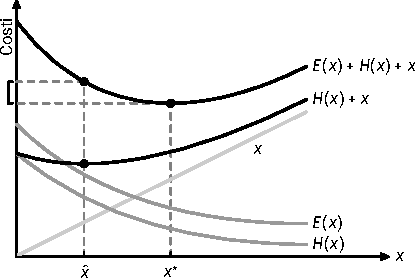
\includegraphics[width=\textwidth]{./figure/esternalita-precauzioni.pdf}
\end{center}
\end{column}
\end{columns}
\end{frame}

%%%%%%%%%%%%%%%%%%%%%%%%%%%%%%%%%%%%%%%%
\begin{frame}{Esternalità e livello di attività}
\begin{columns}
\begin{column}{.5\columnwidth}
In alcuni casi l’esternalità è legata al livello di un'attività. Esempi:
\begin{itemize}
\item le emissioni sono dovute al consumo di carburante e quindi dipendono dalla distanza percorsa da un automezzo;
\item il rischio del verificarsi di un incidente dipende dalle ore di attività di un impianto.
\end{itemize}
L’attività $z$ porta un beneficio $B(z)$ a chi la svolge, ha un costo privato $C(z)$ e un costo sociale $E(z)$.
\end{column}
\begin{column}{.5\columnwidth}
\begin{center}
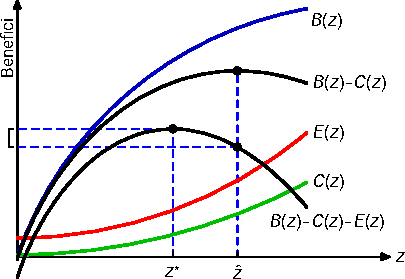
\includegraphics[width=\textwidth]{./figure/esternalita-1-color.pdf}
\end{center}
\end{column}
\end{columns}
\end{frame}

%%%%%%%%%%%%%%%%%%%%%%%%%%%%%%%%%%%%%%%%
\begin{frame}{Dai costi/benefici totali ai costi/benefici marginali}
\begin{columns}
\begin{column}[b]{.5\columnwidth}
\begin{center}
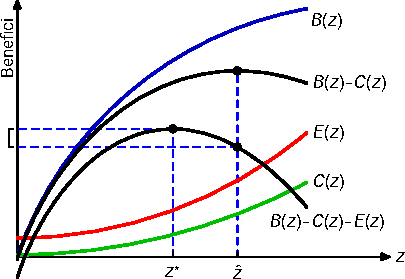
\includegraphics[width=\textwidth]{./figure/esternalita-1-color.pdf}
\end{center}

\vfill

\hfill
\begin{tikzpicture}
\draw[->, line width=2mm,arrows={-Latex[length=5mm,angle'=90]},
      color=blue!30!white] (4,1) to [bend right] (6,0);
\end{tikzpicture}
\end{column}

\begin{column}[b]{.5\columnwidth}
L'individuazione dell'ottimo è più agevole se facciamo riferimento a costi e
benefici marginali.
\vfill

\begin{center}
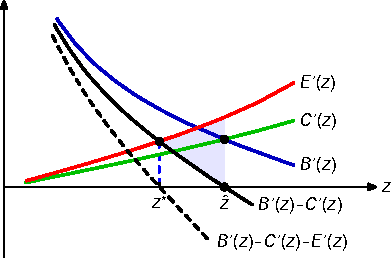
\includegraphics[width=\textwidth]{./figure/esternalita-2-color.pdf}
\end{center}
\end{column}
\end{columns}
\end{frame}

%%%%%%%%%%%%%%%%%%%%%%%%%%%%%%%%%%%%%%%%
\begin{frame}{I costi/benefici marginali: semplifichiamo il grafico}
\begin{columns}
\begin{column}[b]{.5\columnwidth}
\begin{center}
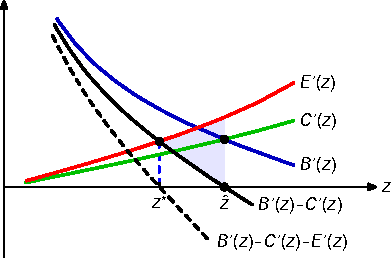
\includegraphics[width=\textwidth]{./figure/esternalita-2-color.pdf}
\end{center}

\vfill

\hfill
\begin{tikzpicture}
\draw[->, line width=2mm,arrows={-Latex[length=5mm,angle'=90]},
      color=blue!30!white] (4,1) to[bend right] (6,0);
\end{tikzpicture}
\end{column}

\begin{column}[b]{.5\columnwidth}
Indichiamo solo il beneficio marginale privato netto BM e il danno marginale esterno DM. È tutto quello che ci serve per identificare $\hat{z}$ e $z^*$.
\vfill

\begin{center}
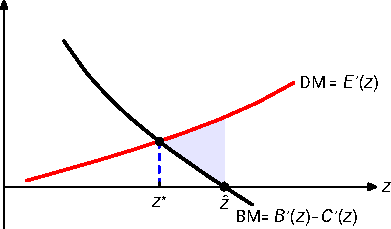
\includegraphics[width=\textwidth]{./figure/esternalita-3-color.pdf}
\end{center}
\end{column}
\end{columns}
\end{frame}

%%%%%%%%%%%%%%%%%%%%%%%%%%%%%%%%%%%%%%%%
\begin{frame}{Il «livello ottimale» di esternalità}
\begin{itemize}
\item Esiste un livello "ottimale" di esternalità che non è necessariamente zero:
\begin{itemize}
\item può non essere ottimale eliminare del tutto l'inquinamento;
\item può non essere ottimale azzerare i rischi di un'attività pericolosa.
\end{itemize}
\item L’analisi economica inquadra il problema come un confronto di costi e
benefici. Ragionando nel continuo vale la consueta analisi al margine
(è ottimale ridurre l'esternalità finché i costi marginali sociali eccedono i costi
marginali di tale riduzione).
\item Il «cinismo» degli economisti si scontra spesso col senso comune:
\begin{itemize}
\item è legittimo pesare costi e benefici anche rispetto a questioni come la
salvaguardia dell'ambiente o la vita delle persone?
\item L’approccio economico, rispetto a divieti e vincoli, predilige soluzioni
che operano sugli incentivi agli individui.
\end{itemize}
\end{itemize}
\end{frame}

\section{I rimedi alla presenza di esternalità negative}


%%%%%%%%%%%%%%%%%%%%%%%%%%%%%%%%%%%%%%%%
\begin{frame}{Come ristabilire l'efficienza?}
\fontsize{13}{16}\selectfont

Le soluzioni più comuni per affrontare il problema delle esternalità negative sono:
\begin{itemize}
\item la \alert{regolazione}, tramite imposizione di obblighi o divieti;
\item la previsione della \alert{responsabilità} di risarcire i danni cagionati con le proprie azioni;
\item la \alert{tassazione} delle attività che generano esternalità negative (imposte «pigouviane»).
\end{itemize}

Spesso più soluzioni sono utilizzate congiuntamente.
\end{frame}

%%%%%%%%%%%%%%%%%%%%%%%%%%%%%%%%%%%%%%%%
\begin{frame}{1. La regolazione}
\begin{itemize}
\item \alert{Regolazione}: imposizione di obblighi e divieti, accompagnati da sanzioni in
caso di mancato adempimento. Esempi:
\begin{itemize}
\item installazione di un impianto antincendio, di un allarme, di una scala di
emergenza, il rispetto di certe procedure e standard, ecc.;
\item un limite di velocità;
\item l’obbligo di revisione periodica di un veicolo;
\item l’obbligo di vaccinazione.
\end{itemize}
\item La regolazione è \alert{efficiente} se le precauzioni cui è tenuto il potenziale
danneggiante è obbligato hanno un costo inferiore al danno atteso che viene
evitato da tali precauzioni.
\item La regolamentazione non può tuttavia tenere conto della situazione
specifica, dei costi e benefici di un certo obbligo in un particolare
contesto; l'approccio \emph{one size fits all} spesso comporta inefficienze:
\begin{itemize}
\item obblighi o divieti che in un certo contesto specifico risultano
eccessivamente onerosi rispetto ai benefici;
\item mancata considerazione di soluzioni alternative meno costose che in quello
specifico contesto potrebbero ridurre il danno.
\end{itemize}
\end{itemize}
\end{frame}

%%%%%%%%%%%%%%%%%%%%%%%%%%%%%%%%%%%%%%%%
\begin{frame}{2. La responsabilità civile}
\begin{itemize}
\item È lo strumento prevalente con cui nella vita di tutti i giorni si realizza
l'internalizzazione delle esternalità.
\item Prevede che
\begin{itemize}
\item in presenza di un danno (non solo potenziale) e
\item di un nesso di causalità tra azione e danno,
\end{itemize}
il danneggiante risarcisca il danneggiato per il danno cagionato.
\item Opera \emph{ex post} rispetto al danno, ma si presume che costituisca un
deterrente a compiere l'azione quando il risarcimento atteso è maggiore dei
benefici dell'azione stessa.
\end{itemize}

\begin{block}{Il punto di vista economico sulla responsabilità civile}
\fontsize{10}{11}\selectfont
\begin{itemize}
\item In un'ottica giuridica spesso si pensa al risarcimento come una forma di
\alert{compensazione delle vittime} per il torto subito.
\item Nell'ottica economica il risarcimento è visto nel suo effetto
disincentivante/deterrente l'azione dannosa.
\item Se l'obiettivo fosse la compensazione, sarebbemeno costoso prevedere forme
di assicurazione (privata o sociale).
\end{itemize}
\end{block}
\end{frame}

%%%%%%%%%%%%%%%%%%%%%%%%%%%%%%%%%%%%%%%%
\begin{frame}{La responsabilità civile è sufficiente?}
\begin{itemize}
\item Non sempre la responsabilità civile è sufficiente ad indurre un livello
efficiente di esternalità:
\begin{itemize}
\item se il danneggiato non conosce l'identità del danneggiante (magari perché il
danneggiante si nasconde, caso probabile nel caso di azione dolosa);
\item se il nesso di causalità non è chiaro;
\item intraprendere l'azione legale è costoso: l'incentivo privato ad
intraprendere l'azione legale (costi/benefici derivanti dal risarcimento al
netto dei costi legali) non è allineato con quello sociale (rappresentato
dalla deterrenza);
\item il danneggiante può non essere consapevole degli effetti potenzialmente
dannosi delle sue azioni;
\item il patrimonio del danneggiante potrebbe non essere capiente (vedi oltre).
\end{itemize}
\item In queste circostanze è preferibile \alert{prevenire} il verificarsi del danno
attraverso la regolazione oppure la tassazione* dei comportamenti
potenzialmente dannosi.
\end{itemize}
\end{frame}

%%%%%%%%%%%%%%%%%%%%%%%%%%%%%%%%%%%%%%%%
\begin{frame}{3. La tassazione (e il sussidio)}
\begin{itemize}
\item In alternativa alla fissazione di limiti espliciti, è possibile indurre un
comportamento corretto puntando a far internalizzare il costo sociale
dell'esternalità tramite imposte (imposte «pigouviane», da A. C. Pigou).
\item Esempi:
\begin{itemize}
\item imposte sui combustibili fossili;
\item \emph{Carbon Tax};
\item altre «sin taxes» (alcolici, tabacco, «sugar tax», «fat tax»\ldots{}).
\end{itemize}
\item L'imposta pigouviana consente alle imprese di scegliere il livello adeguato
in funzione delle specifiche condizioni di produzione (può richiedere meno
informazioni).
\item A differenza di regolazione e responsabilità civile, le imposte pigouviane
sono in grado di indurre non solo un livello efficiente di precauzioni, ma
anche un efficiente \alert{livello di attività}.
\end{itemize}
\end{frame}

%%%%%%%%%%%%%%%%%%%%%%%%%%%%%%%%%%%%%%%%
\begin{frame}{La tassazione e livello ottimale di attività}
\begin{itemize}
\item Poniamo che benefici e costi sociali dipendano sia dal livello di
precauzioni $x$ che dal livello di attività svolta $z$:
\begin{equation*}
b(z) - z[c+x] - p(x)zh
\end{equation*}
dove:
\begin{itemize}
\item $z$ è il livello di attività (produzione),
\item $b(z)$ è il beneficio privato dell'attività,
\item $c + x$ il costo unitario dell’attività $x$, che dipende dal livello di
precauzioni $x$.
\end{itemize}
\item Anche fissando correttamente x (con regolazione o responsabilità per colpa,
che punisce un comportamento negligente), il livello di $z$ non sarebbe scelto
correttamente.
\item Un'imposta commisurata a $z$ può ristabilire l’efficienza.
\begin{itemize}
\item Qual è l’ammontare ottimale dell’imposta?
\end{itemize}
\item In alternativa: la responsabilità oggettiva.
\end{itemize}
\end{frame}

%%%%%%%%%%%%%%%%%%%%%%%%%%%%%%%%%%%%%%%%
\begin{frame}{(4.) L'attribuzione di permessi negoziabili (\emph{cap \& trade})}
\begin{itemize}
\item Applicato nel caso delle emissioni inquinanti, come strumento per limitare i gas serra;
\item come nella regolazione, si fissa il livello di attività o di inquinamento, ma tale limite è definito a livello complessivo;
\item si attribuisca alle imprese una certa quantità di "permessi" di svolgere l'attività (e quindi di inquinare);
\item si consente alle imprese di vendere e acquistare tali permessi, (acquisterà permessi chi trae maggior vantaggio dall'inquinamento e/o sostiene un costo maggiore per ridurre le emissioni);
\item il «mercato dei permessi» alloca i diritti a inquinare in modo efficiente (a parità di inquinamento si produce maggiore valore).
\end{itemize}
\end{frame}

\section{La prospettiva di Coase e la negoziazione dei diritti}

%%%%%%%%%%%%%%%%%%%%%%%%%%%%%%%%%%%%%%%%
\begin{frame}{Pigou vs Coase}
\begin{columns}
\begin{column}{.5\columnwidth}
\begin{itemize}
\item Arthur C. Pigou (1877-1959) suggerì interventi correttivi dello stato nella
forma di imposte ("\alert{pigouviane}") sulle attività che producono esternalità
negative e sussidi alle attività che producono esternalità positive.
\end{itemize}
\begin{figure}[htbp]
\centering
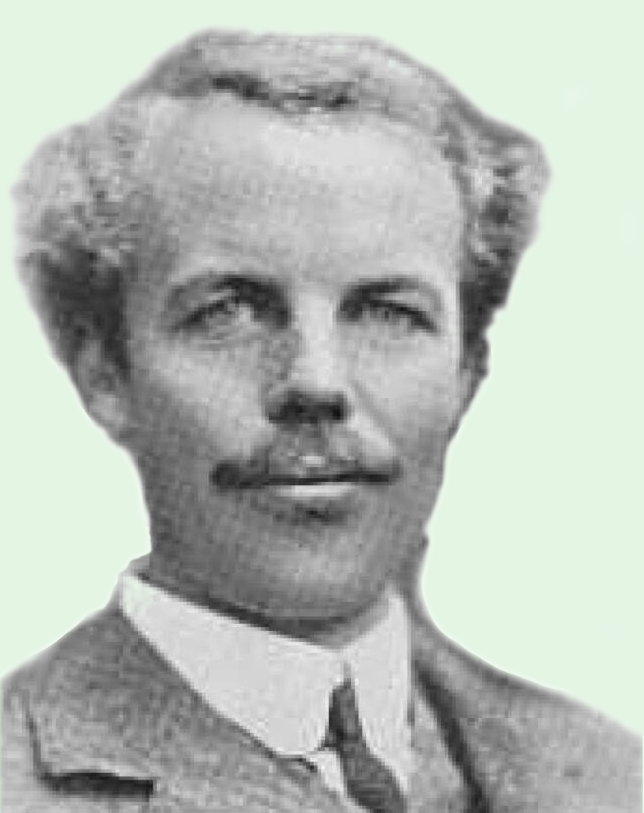
\includegraphics[height=4cm]{./figure/Pigou.png}
\end{figure}
\end{column}
\begin{column}{.5\columnwidth}
\begin{itemize}
\item La visione di Pigou fu messa in discussione da Ronald Coase (1910-2013), con
un famoso articolo uscito nel 1960 («The problem of social cost»).
\end{itemize}
\begin{figure}[htbp]
\centering
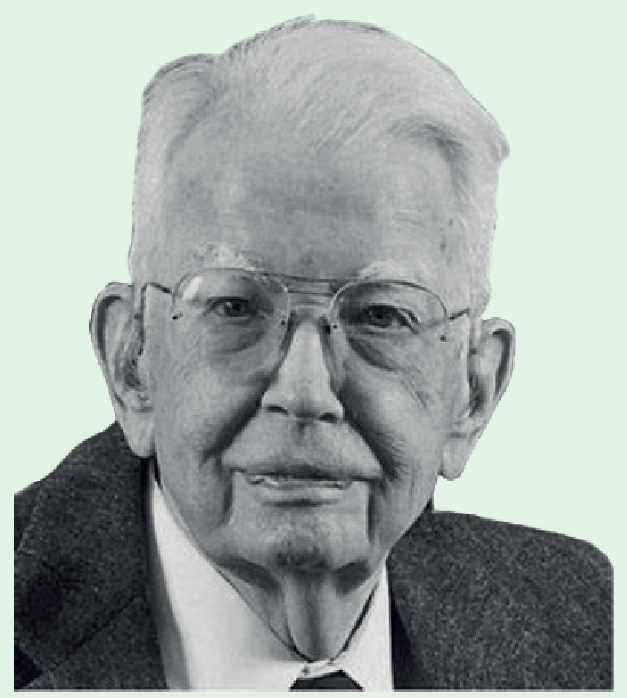
\includegraphics[height=4cm]{./figure/Coase.png}
\end{figure}
\end{column}
\end{columns}
\end{frame}

%%%%%%%%%%%%%%%%%%%%%%%%%%%%%%%%%%%%%%%%
\begin{frame}{Le natura reciproca delle esternalità}
\begin{itemize}
\item È bene considerare le esternalità come qualcosa di «reciproco»:
\begin{itemize}
\item l'attività inquinante di A danneggia B
\item \ldots{}ma la rinuncia ad inquinare B procura un danno ad A!
\end{itemize}
\item La «direzione» dell'esternalità dipende dall'allocazione iniziale dei
diritti (diritto a svolgere una certa attività, diritto a non essere
danneggiato).
\item Possiamo chiederci quale allocazione dei diritti sia più «efficiente¢, in
base ai costi sostenuti dalle diverse parti coinvolte:
\begin{itemize}
\item l'allocazione dei diritti di proprietà ha effetto distributivo e di
efficienza;
\item Coase sottolinea che la riallocazione dei diritti può avere luogo in modo
«decentrato»;
\item le esternalità possono essere considerate un problema di "assenza di
mercato", ma se le parti potessero "creare" il mercato\ldots{}
\end{itemize}
\end{itemize}
\end{frame}

%%%%%%%%%%%%%%%%%%%%%%%%%%%%%%%%%%%%%%%%
\begin{frame}{Il teorema di Coase}
\vspace*{-2mm}
\begin{block}{}
Se i costi di transazione sono trascurabili, le parti si accorderanno per
l'adozione di una soluzione efficiente indipendentemente dall'attribuzione
iniziale dei diritti di proprietà.
\end{block}
\begin{itemize}
\item Non sempre è necessario un intervento pubblico correttivo.  Lo Stato può
limitarsi a definire i diritti e garantirne il rispetto.
\item Il teorema di Coase è una \emph{tautologia}? Afferma che se è possibile
accordarsi per esito efficiente, avremo un esito efficiente\ldots{}
\end{itemize}

Più interessante se lo si formula diversamente:
\vspace{-2mm}
\begin{block}{}
In assenza di costi di transazione l'allocazione dei diritti di proprietà
(diritto ad inquinare o a non essere inquinato) è irrilevante ai fini del
raggiungimento dell'efficienza.
\end{block}
\begin{itemize}
\item Dunque, leggendolo «in negativo»: è la presenza dei costi di transazione
che «spiega» la preferibilità di certe soluzioni giuridiche (allocazione
di diritti) rispetto ad altre.
\end{itemize}
\end{frame}

%%%%%%%%%%%%%%%%%%%%%%%%%%%%%%%%%%%%%%%%
\begin{frame}{Un esempio}
\begin{itemize}
\item Una segheria molto rumorosa è situata accanto a una bellissima spiaggia dove
sarebbe possibile realizzare un resort:
\begin{itemize}
\item la mancata realizzazione del resort comporta mancato profitto pari a 2.000;
\item lo spostamento della segheria comporta costo pari a 1.000.
\end{itemize}
Pertanto, sarebbe efficiente spostare la segheria.
\item La negoziazione consentirebbe alle parti di raggiungere l'esito efficiente.
\item In mancanza di negoziazione, l'attribuzione del diritto a un soggetto o
  all'altro incide sull'esito in termini di valore complessivo.
\item In conclusione: è efficiente che il diritto sia assegnato al soggetto
  che gli attribuisce il più alto valore, ma non sempre tale soggetto può
  segnalarlo attraverso il mercato!
\end{itemize}
\end{frame}

%%%%%%%%%%%%%%%%%%%%%%%%%%%%%%%%%%%%%%%%
\begin{frame}{Proprietà comune, inalienabilità e altri limiti alla negoziazione}
\begin{itemize}
\item In molti casi la negoziazione non ha luogo perché il diritto interessato
dall'esternalità è di natura collettiva (proprietà comune, congestione,
ecc.)
\item Una possibile soluzione: il passaggio ad una proprietà individuale della
risorsa.
\begin{itemize}
\item Esempio: proposte di limitare la deforestazione "privatizzando" le foreste
\end{itemize}
\item In molti casi non è possibile o è troppo costoso negoziare prima che
l'esternalità abbia luogo. Esempio: incidenti stradali o altri eventi
accidentali che danneggiano terzi non identificabili in anticipo
\begin{itemize}
\item In questi casi opera la responsabilità civile: se A compie un'azione che
lede il diritto di B, deve risarcirlo per il danno cagionato, a un prezzo
stabilito ex post dagli avvocati o dal giudice
\end{itemize}
\item In altri casi la cessione del diritto (a titolo oneroso ma anche gratuito)
non è considerata socialmente/politicamente accettabile. Il diritto è
inalienabile.
\begin{itemize}
\item diritto all'integrità fisica.
\end{itemize}
\item Conflitto tra efficienza e morale (M. Sandel, I limiti sociali del mercato)
\end{itemize}
\end{frame}

%%%%%%%%%%%%%%%%%%%%%%%%%%%%%%%%%%%%%%%%
\begin{frame}{Mercato e morale}
\begin{columns}
\begin{column}{.6\columnwidth}
\begin{itemize}
\item L'acquisto del diritto a non essere arruolati nell’esercito federale durante
la Guerra civile americana.
\item L'acquisto di un posto con maggiore priorità nella lista di attesa per un
trapianto
\item La vendita dei propri organi in caso di decesso.
\item ecc.
\end{itemize}
\end{column}

\begin{column}{.4\columnwidth}
\begin{center}

\includegraphics[width=\textwidth]{./figure/Sandel-limiti-morali.jpeg}
\end{center}
\end{column}
\end{columns}
\end{frame}

\section{La scelta dello strumento più appropriato}


%%%%%%%%%%%%%%%%%%%%%%%%%%%%%%%%%%%%%%%%
\begin{frame}{Una confronto tra i possibili rimedi}
\begin{itemize}
\item I rimedi alla presenza di esternalità possono essere distinti:
\begin{itemize}
\item in base al fatto che guardino alle azioni potenzialmente dannose (ex ante) o
al verificarsi del danno (ex post)
\item in base al fatto che la «sanzione» sia incondizionata o condizionata al
rispetto di uno standard prefissato
\end{itemize}
\end{itemize}

\begin{center}
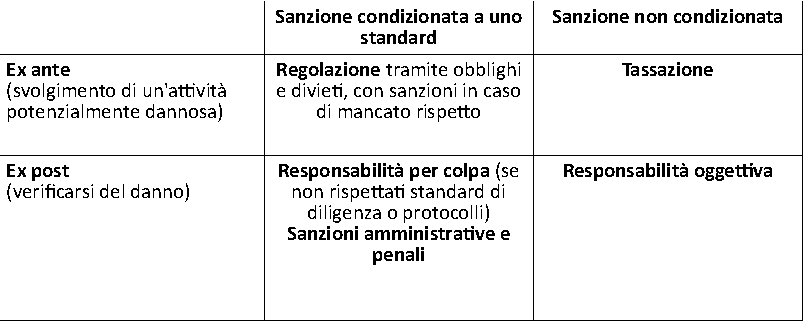
\includegraphics[width=.9\linewidth]{./figure/esternalita-comparazione-rimedi.pdf}
\end{center}
\end{frame}


%%%%%%%%%%%%%%%%%%%%%%%%%%%%%%%%%%%%%%%%
\begin{frame}{Ex post o ex ante? Il problema dell'incapienza}
\begin{itemize}
\item Nei casi in cui bassa probabilità di un danno estremamente elevato (es. petroliere, centrali nucleari)
\item Ipotizziamo che, in assenza di precauzioni (il cui costo è 100), aumenti dell'1\% la probabilità di un danno pari a 20.000. In questo caso è efficiente sostenere il costo delle precauzioni
\item Con la responsabilità civile, il risarcimento atteso è pari al danno atteso:\\[0pt]
$20.000 \times 1\% = 200$, quindi c'è incentivo a prendere le precauzioni
\item Se tuttavia il patrimonio del danneggiante è pari a 8.000, il costo atteso
diventa:\\[0pt]
$8.000 \times 1\% = 80 < 100$ e non si prenderanno le precauzioni
\item Può essere conveniente imporre le precauzioni e sanzionare il mancato
assolvimento di questo obbligo
\begin{itemize}
\item Esempio: senza le dovute precauzioni, probabilità del 10\% di un controllo;
basta una multa superiore a 1.000 per indurre un comportamento corretto
\item bisogna tuttavia tenere conto del costo di controlli\ldots{}
\end{itemize}
\end{itemize}
\end{frame}

%%%%%%%%%%%%%%%%%%%%%%%%%%%%%%%%%%%%%%%%
\begin{frame}{Standard o sanzione incondizionata?}
\begin{itemize}
\item La soluzione della regolamentazione in questo caso consiste nell'imposizione
di un \alert{limite massimo} al livello di attività/esternalità
\item Potendo osservare e misurare l'attività/esternalità, una soluzione
alternativa è la \alert{tassazione} dell'esternalità (anche indirettamente,
tassando un input o output la cui quantità è direttamente correlata
all'esternalità)
\end{itemize}

\begin{columns}
\begin{column}{.5\columnwidth}
\begin{itemize}
\item Se dunque la regolamentazione consiste in un limite massimo $w^*$, la
tassazione impone il pagamento di un imposta proporzionale a $w$ con
aliquota $t$
\item Sia la quantità $w^*$ che l'aliquota $t$ sono calcolate con riferimento
al livello efficiente, cioè al punto F
\item Le due soluzioni sono equivalenti se il punto F è noto. Ma se è incerto?
\end{itemize}
\end{column}
\begin{column}{.5\columnwidth}
\begin{figure}
\centering
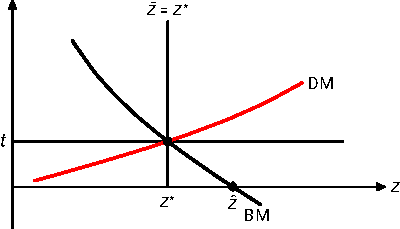
\includegraphics[width=\textwidth]{./figure/esternalita-5-color.pdf}
\end{figure}
\end{column}
\end{columns}
\end{frame}

%%%%%%%%%%%%%%%%%%%%%%%%%%%%%%%%%%%%%%%%
\begin{frame}{Regolazione e tassazione in presenza di incertezza}
\begin{itemize}
\item Ipotizziamo che vi sia incertezza riguardo al beneficio marginale netto BMN
\begin{itemize}
\item il regolatore non conosce costi/benefici per l'impresa di variare il
livello di esternalità. La curva stimata BMN$^*$ può essere diversa dalla
curva effettiva BMN.
\end{itemize}
\item Quale soluzione minimizza il costo dell'errore? Dipende
\end{itemize}
\begin{columns}
\begin{column}{.5\columnwidth}
\begin{figure}
\centering
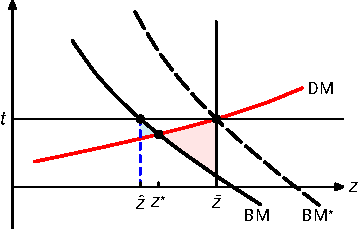
\includegraphics[width=\textwidth]{./figure/esternalita-6-color.pdf}
La regolamentazione è preferibile
\end{figure}
\end{column}

\begin{column}{.5\columnwidth}
\begin{figure}
\centering
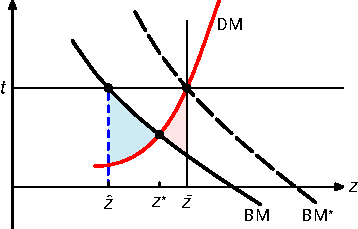
\includegraphics[width=\textwidth]{./figure/esternalita-7-color.pdf}
La tassazione è preferibile
\end{figure}
\end{column}
\end{columns}
\end{frame}


%%%%%%%%%%%%%%%%%%%%%%%%%%%%%%%%%%%%%%%%
\begin{frame}{Regolazione e tassazione in presenza di incertezza /2}
\begin{itemize}
\item \alert{La tassazione è preferibile} quando il danno atteso cresce (grosso modo)
proporzionalmente con l'aumentare del livello di esternalità/attività (curva
di danno marginale sociale DM piatta)
\begin{itemize}
\item In questo caso, il fatto che il regolatore non conosca il livello
efficiente di esternalità non è un problema, perché sarà il danneggiante
aggiusterà la quantità in base alla propria curva BM
\end{itemize}

\item \alert{La regolazione è preferibile} quando è facilmente stimabile il livello
efficiente di esternalità/attività e tale stima non risente in modo
significativo dell'incertezza sul beneficio marginale privato (cioè della
posizione della curva BM)
\begin{itemize}
\item Es. effetti «soglia», danno marginale sociale elevato al di sopra di un
certo livello (curva del danno marginale sociale «a gradino»)
\item la tassazione non è in grado di garantire che il livello di esternalità
non superi la soglia
\end{itemize}
\end{itemize}
\end{frame}

%%%%%%%%%%%%%%%%%%%%%%%%%%%%%%%%%%%%%%%%
\begin{frame}{La regolamentazione: \emph{one size fits all}?}
\begin{itemize}
\item Un ulteriore svantaggio della regolamentazione è che essa tende ad imporre
vincoli uniformi a situazioni diverse (\emph{one size fits all})
\end{itemize}

\begin{columns}
\begin{column}{.5\columnwidth}
\begin{itemize}
\item Due imprese con diverso beneficio marginale.
\item Fissando un livello di esternalità comune per le due imprese, non si è in
grado di indurre un livello efficiente per entrambe;
\item la perdita di benessere è rappresentata dalle due aree ombreggiate.
\end{itemize}
\end{column}

\begin{column}{.5\columnwidth}
\begin{figure}[htbp]
\centering
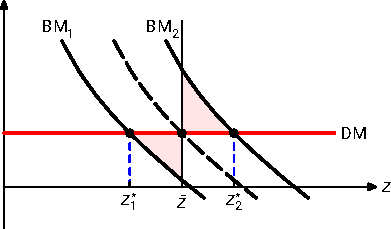
\includegraphics[width=\textwidth]{./figure/esternalita-8-color.pdf}
\end{figure}
\end{column}
\end{columns}
\end{frame}

%%%%%%%%%%%%%%%%%%%%%%%%%%%%%%%%%%%%%%%%
\begin{frame}{La tassazione non soffre dello stesso problema}
\begin{columns}
\begin{column}{.5\columnwidth}
\begin{figure}[htbp]
\centering
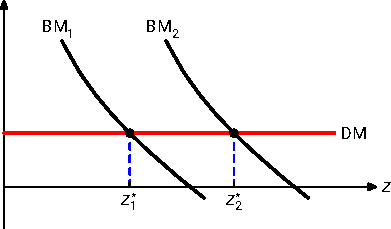
\includegraphics[width=\textwidth]{./figure/esternalita-9-color.pdf}
\end{figure}
\end{column}
\begin{column}{.5\columnwidth}
\begin{itemize}
\item Ipotizzando che il DM sia costante, fissiamo l'aliquota $t$
sull'attività/esternalità ad un livello pari al danno marginale DM
(calcolato in corrispondenza del livello di esternalità desiderato)
\item Le due imprese, sulla base dei rispettivi BMN, sceglieranno i livelli
efficienti di esternalità $w_1$ e $w_2$
\item Possiamo immaginare la tassazione come una «vendita» del diritto ad
inquinare ad un prezzo prefissato (l'aliquota di imposta)
\end{itemize}
\end{column}
\end{columns}
\end{frame}

%%%%%%%%%%%%%%%%%%%%%%%%%%%%%%%%%%%%%%%%
\begin{frame}{Vincoli o incentivi? La dimensione distributiva}
\begin{itemize}
\item Vincoli uniformi impongono uno stesso obbligo o divieto indipendentemente
dal costo/beneficio individuale. Gli incentivi incoraggiano gli individui a
confrontare costi e benefici
\begin{itemize}
\item In presenza di un divieto, la sanzione può essa stessa essere considerata
come il «prezzo» per la violazione di una norma
\end{itemize}
\item Dal punto di vista dell’efficienza, non è ottimale eliminare un’esternalità
se il danno sociale è inferiore al beneficio marginale per il danneggiante
\item È accettabile che individui per i quali il beneficio associato a
un’esternalità è maggiore possano violare una norma perché hanno una
maggiore disponibilità a pagare?
\begin{itemize}
\item pagare la contravvenzione per parcheggiare la Porsche in piazza Duomo
\item dobbiamo vietare l’uso dei jet privati?
\end{itemize}
\item È «equo» modulare la sanzione in base alla ricchezza? O è preferibile
intervenire direttamente sulla distribuzione del reddito e lasciare che la
regolazione delle esternalità sia improntata al solo criterio
dell’efficienza?
\end{itemize}
\end{frame}

%%%%%%%%%%%%%%%%%%%%%%%%%%%%%%%%%%%%%%%%
\begin{frame}{La soluzione del \emph{cap and trade}}
\begin{itemize}
\item Il problema dato dall'impossibilità di personalizzare i limiti può essere
superato consentendo alle imprese di scambiare i diritti ad inquinare (\emph{cap
and trade})
\item Una volta fissato il livello obiettivo aggregato $W$ di esternalità, tale
livello viene suddiviso tra le imprese (secondo un criterio qualunque, ad
esempio in quote uguali o in base ai livelli storici di inquinamento)
\item le imprese possono scambiarsi i permessi di emissione---si crea un mercato
dei permessi in cui le imprese che assegnano (al margine) maggior valore al
permesso lo acquistano da quelle che assegnano minor valore
\item in equilibrio tutte le imprese fisseranno un livello di emissione tale che
il BM$^{h}$ (beneficio marginale netto) è pari a tale prezzo $p$ (e quindi è
lo stesso per tutte le imprese)
\end{itemize}
\begin{block}{}
Se il prezzo finale è $p=DM$, significa che DM=BM per ciascuna impresa:
livello e allocazione delle emissioni sono dunque efficienti.

Che significato diamo al fatto che in equilibrio possa essere $p>\text{DM}$
oppure $p<\text{DM}$?
\end{block}
\end{frame}


%%%%%%%%%%%%%%%%%%%%%%%%%%%%%%%%%%%%%%%%
\begin{frame}{Tassazione o \emph{cap \& trade}?}
\begin{itemize}
\item Sia la tassazione che il \emph{cap and trade} conducono ad un'allocazione
efficiente delle emissioni, pur in presenza di imprese inquinanti
eterogenee.
\end{itemize}
I due sistemi presentano tuttavia delle differenze:
\begin{itemize}
\item \alert{con la tassazione}, fisso d'autorità il "prezzo/imposta" che guiderà le
scelte delle imprese, ma non sono certo a priori della quantità di
inquinamento, che dipenderà dalle scelte delle imprese
\begin{itemize}
\item se la quantità è maggiore (minore) delle attese, posso correggere alzando
(abbassando) il prezzo
\end{itemize}
\item \alert{con il \emph{cap and trade}}, posso controllare in anticipo l'ammontare totale
di emissioni, e sarà il mercato a determinare il "prezzo" di un'unità di
inquinamento
\begin{itemize}
\item se il prezzo risulta inferiore al danno marginale sociale (cioè le imprese
attribuiscono ai diritti ad inquinare un valore inferiore al loro costo
sociale) sarà opportuno ridurre il livello obiettivo [sapreste spiegare
perché?]
\end{itemize}
\item Le due soluzioni differiscono anche negli esiti distributivi, visto che nel
caso della tassazione le imprese pagano per inquinare, nel caso \emph{cap and
trade} pagano o sono pagate quando scambiano diritti
\begin{itemize}
\item Per effettuare correttamente il confronto occorre conoscere la
destinazione delle imposte
\end{itemize}
\end{itemize}
\end{frame}

%%%%%%%%%%%%%%%%%%%%%%%%%%%%%%%%%%%%%%%%
\begin{frame}{Le esternalità ambientali in pratica}
\begin{itemize}
\item Gli esempi più rilvanti di \alert{cap and trade} sono gli schemi di \alert{emission trading} per l'attuazione del protocollo di Kyoto di riduzione dei gas serra
\begin{itemize}
\item \url{https://en.wikipedia.org/wiki/Emissions\_trading} su Wikipedia (in inglese)
\item \url{http://www.minambiente.it/pagina/direttiva-emission-trading} sul sito del
Min. dell'Ambiente
\end{itemize}
\item In alternativa la soluzione della \alert{carbon tax}
\begin{itemize}
\item \url{https://it.wikipedia.org/wiki/Carbon\_tax}
\end{itemize}
\item In tema di ambiente e inquinamento, due casi eclatanti di ricorso alla responsabilità civile sono stati
\begin{itemize}
\item Il processo alla Exxon per il naufragio della superpetroliera Exxon-Valdez nel Golfo dell'Alaska nel 1989, conclusosi con il più alto risarcimento mai registrato per un disastro industriale
\item Il processo per il Petrolchimico di Porto Marghera (causa civile e penale)
\end{itemize}
\end{itemize}
\end{frame}

%%%%%%%%%%%%%%%%%%%%%%%%%%%%%%%%%%%%%%%%
\begin{frame}{Riassumendo: i rimedi alle esternalità negative}
\begin{itemize}
\item Abbiamo visto che esiste una pluralità di rimedi al problema delle esternalità negative:
\begin{itemize}
\item attribuzione dei diritti di proprietà
\item responsabilità civile
\item regolamentazione
\item tassazione
\end{itemize}
\item La tassazione non è lo strumento più diffuso, ma vi sono molti esempi rilevanti di tassazione di beni/attività che producono esternalità:
\begin{itemize}
\item tassazione sui combustibili fossili è parte rilevante del prezzo della
benzina
\item tassazione sul tabacco (ma è esternalità o "internalità"?)
\item in molti paesi tassazione elevata sugli alcolici
\item a livello locale: \emph{congestion charge}
\end{itemize}
\item la finalità è quella di scoraggiare le attività che generano esternalità facendo internalizzare il costo---ciò non esclude che vi sia anche una motivazione di \emph{gettito}
\end{itemize}
\end{frame}

\section{Le sanzioni: un'analisi economica}

%%%%%%%%%%%%%%%%%%%%%%%%%%%%%%%%%%%%%%%%
\begin{frame}{L'applicazioni di sanzioni pecuniarie e non pecuniarie}
\begin{itemize}
\item In alcuni casi applicazione di sanzioni per violazione di norma
(eventualmente subordinata al verificarsi di un danno)
\item Sanzioni \alert{pecuniarie} o \alert{non pecuniarie} (carcere, interdizione dallo
svolgimento dell'attività, ritiro della patente, sequestro del veicolo\ldots{})
\item La sanzione pecuniaria è più \alert{efficiente} (non comporta consumo di risorse)
\item Cosa giustifica l'uso di sanzioni non pecuniarie:
\begin{itemize}
\item incapienza del patrimonio del danneggiante
\item "segnalano" la gravità dell'atto
\item associate ad uno "stigma sociale"
\item effetto incapacitante della sanzione non pecuniaria (ma questo non spiega
molti casi di applicazione)
\end{itemize}
\end{itemize}
\end{frame}

%%%%%%%%%%%%%%%%%%%%%%%%%%%%%%%%%%%%%%%%
\begin{frame}{Sanzione elevata o elevata probabilità di sanzionamento?}
\begin{itemize}
\item Sanzioni applicate con probabilità inferiore a 1: ciò che conta è la
\alert{sanzione attesa}
\item Se individuo non avverso al rischio, costo della sanzione è $S=\pi F$ dove
$F$ è la sanzione e $\pi$ è la probabilità di sanzionamento
\begin{itemize}
\item che succede se l'individuo è avverso al rischio?
\end{itemize}
\item Stesso livello di deterrenza con diverse combinazioni di $\pi$ e $F$ (a
parità di $S=\pi F$)
\item Becker: dal punto di vista sociale conviene aumentare $F$ e ridurre $\pi$
\item Perché questo non accade in realtà?
\begin{itemize}
\item equità della sanzione
\item la sanzione come "prezzo" che guida la scelta di quale infrazione
commettere
\item difficile modulare/osservare $\pi$
\end{itemize}
\item La sanzione come \alert{prezzo}: il caso degli asili di Haifa
\end{itemize}
\end{frame}

\section{Esternalità positive}

%%%%%%%%%%%%%%%%%%%%%%%%%%%%%%%%%%%%%%%%
\begin{frame}{Esternalità positive}
\begin{itemize}
\item In questo caso l'esternalità si aggiunge, non si sottrae, al BM privato, per cui il livello efficiente risulta \alert{superiore} al livello scelto
\item Molte delle cose dette per le esternalità valgono anche per il caso di esternalità positive:
\begin{itemize}
\item l'attribuzione di diritti di proprietà è una soluzione---es. proprietà intellettuale su attività innovative e creative
\item obblighi di fare (es. vaccinazioni obbligatorie)
\item sussidi allo svolgimento di attività che generano esternalità positive (esempio incentivi al risparmio energetico, all'installazione di pannelli fotovotaici ecc.)
\end{itemize}
\item in molti casi il sussidio prende la forma di applicazione di \alert{aliquote ridotte} per i beni che comportano esternalità e deduzioni/detrazioni dall'imposta sul reddito per spese meritorie (vedi più avanti)
\end{itemize}
\end{frame}

%%%%%%%%%%%%%%%%%%%%%%%%%%%%%%%%%%%%%%%%
\begin{frame}{Esternalità positive: detrazioni IRPEF 19\%}
\begin{figure}[htbp]
\centering
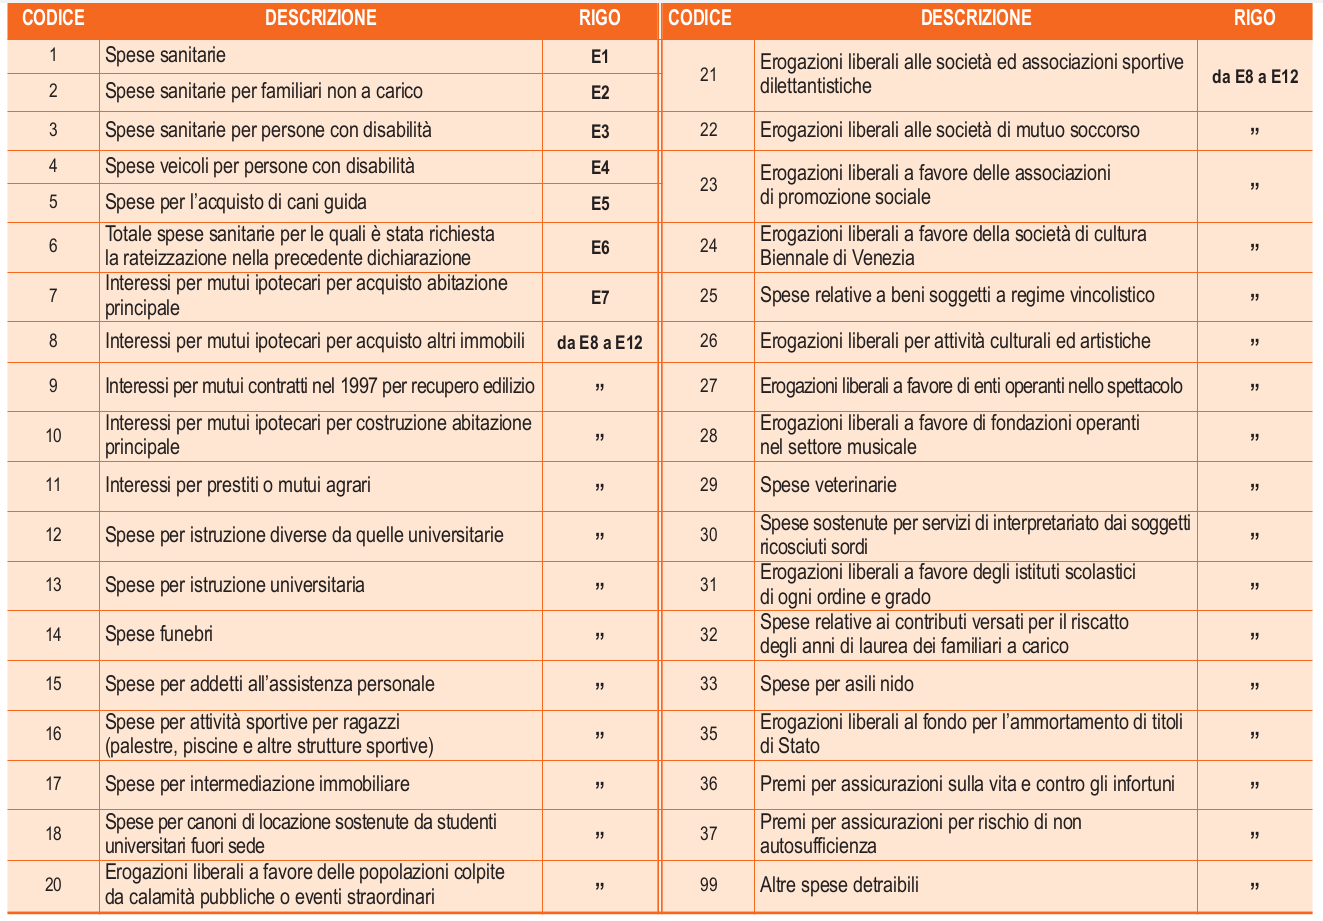
\includegraphics[height=8cm]{./figure/detrazioni-spese-730.png}
\end{figure}
\end{frame}
\end{document}